\section{Speech-Act Misalignment}
\label{sec:speech_act_misalignment}

In the baseline architecture, agent communication relies on perfect information transfer. When a speaker generates a speech act, the resulting payload encapsulates both the natural language text and the exact symbolic parameters:
$$ \texttt{speech(Message, Performative(Target))} $$ 
Because the receiving agent is handed the explicit \textit{Performative} and \textit{Target} by design, pragmatic misunderstanding is structurally impossible. 

\begin{figure}[H]
    \centering
    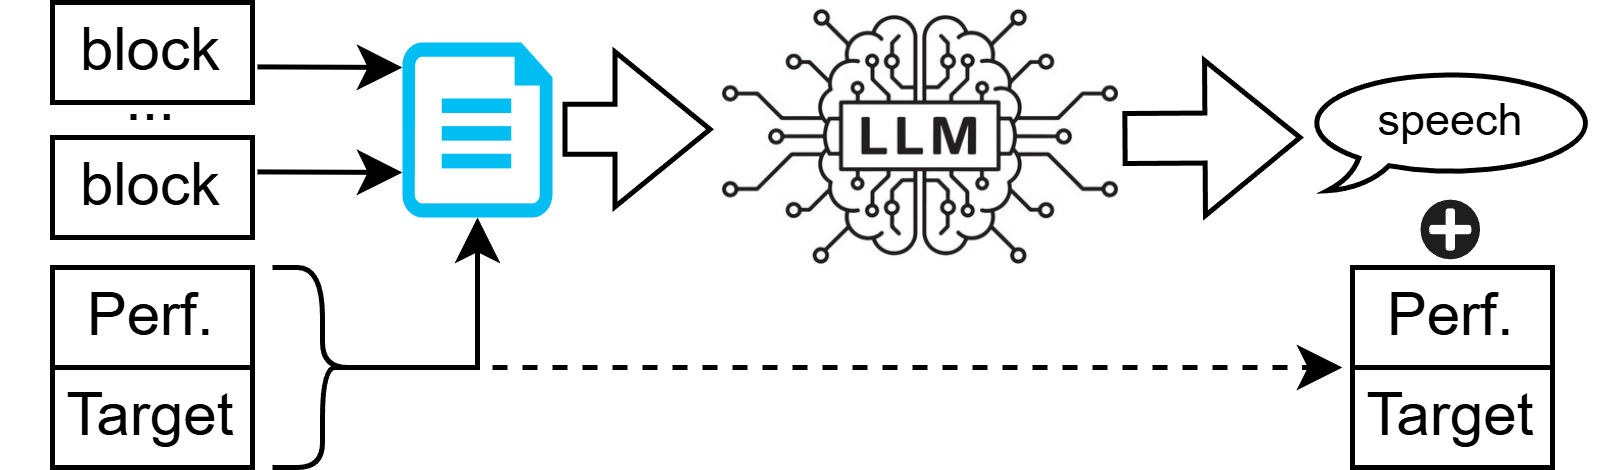
\includegraphics[width=0.6\textwidth]{images/NLP/llm_speech.png}
    \caption{The Natural Language Generation pipeline: the agent first defines the performative and target prior to LLM generation, then it embeds the generated text along with the Speech Act labels.}
    \label{fig:standard_speech_creation}
\end{figure}

To accurately simulate natural human communication (inherently ambiguous), we modify the communication protocol by stripping the symbolic labels during transmission. The receiving agent is now provided strictly with the raw natural language $Message$ and must autonomously retrieve the performative and target.

Given this challenge, we are now faced with a \textbf{Speech-Act Misalignment} problem, and the goal is to limitate it as much as possible, by correctly inferring the performative and the target of a given speech act, by looking at the raw text only.

\subsection{Closed World Assumption}

Extracting pragmatic intent and entity references from open-ended dialogue is an inherently complex NLP task. To ensure computational tractability and allow for a supervised classification architecture, we enforce a Closed World Assumption utilizing three strict constraints:

\begin{itemize}
    \item \textbf{Fixed Performative Domain:} The set of allowed performatives is statically defined and invariant across all games.
    \item \textbf{Fixed Target Domain:} The roster of potential targets is globally restricted to a known, static set of players. This allows the model to predict across a fixed-dimension probability distribution (one-hot encoding) rather than relying on a computationally expensive generative pipeline.
    \item \textbf{Explicit, Singular Targeting:} Every speech act must explicitly name exactly one valid target within the text\footnote{Nonetheless, while the correct target of the  speech is only one, in the text could appear other candidates; without this inconvenient, the problem could perfectly be addressed by a simple regex-based extraction}. This restriction intentionally bypasses the need for complex coreference resolution or implicit entity linking, and ensures maximal recall on target extraction by treating it as a deterministic token lookup task.
\end{itemize}


\paragraph{Dataset Partitioning and Generation}
The training and validation sets were generated using the \texttt{Gemma4:31b} model. To prevent majority-class bias during optimization, both sets were strictly balanced to ensure a uniform joint distribution across all (\textit{Performative}, \textit{Target}) pairs. This yielded a structured dataset of approximately 2,000 tuples for training and 500 tuples for validation. Due to this strict uniform balancing, a naive baseline model evaluated on these sets achieves an expected accuracy of exactly $16.67\%$ ($1/6$) for the performative head and $6.67\%$ ($1/15$) for the target head.

To rigorously evaluate the model's generalization capabilities and verify that the network did not merely overfit the output of a single generative model, evaluation was conducted on two distinct test sets. Each test set was constructed by simulating 50 full games and intentionally preserved the unbalanced frequency of speech acts naturally occurring in the game:
\begin{itemize}
    \item \textbf{In-Distribution Test Set:} $\approx$ 2,500 tuples generated using \texttt{Gemma4:31b}.
    \item \textbf{Cross-Model Test Set:} $\approx$ 2,500 tuples generated using \texttt{Qwen3.5:35b}, serving as a zero-shot robustness check against variations in LLM syntax and phrasing.
\end{itemize}


\subsection{Baseline 1: Anchor-Based Similarity Classification}

To establish an initial baseline, we implemented a zero-shot, similarity-based classification pipeline using the pre-trained \texttt{bert-base-uncased} model \cite{devlin-etal-2019-bert, wolf-etal-2020-transformers}. 

As alredy discussed, each performative is defined by a natural language description (Section \ref{subsubsec:llm-reasoner-encoding}). By instantiating these 6 base descriptions with the names of the 15 possible players, is possible to generated a set of 90 \textit{anchor sentences}. The underlying hypothesis was that the contextual embedding of a generated game message would exhibit high cosine similarity to the specific anchor that prompted it, allowing us to infer the labels via nearest-neighbor matching.

\begin{figure}[H]
    \centering
    % Left side: KDE Distributions
    \begin{subfigure}[b]{0.48\textwidth}
        \centering
        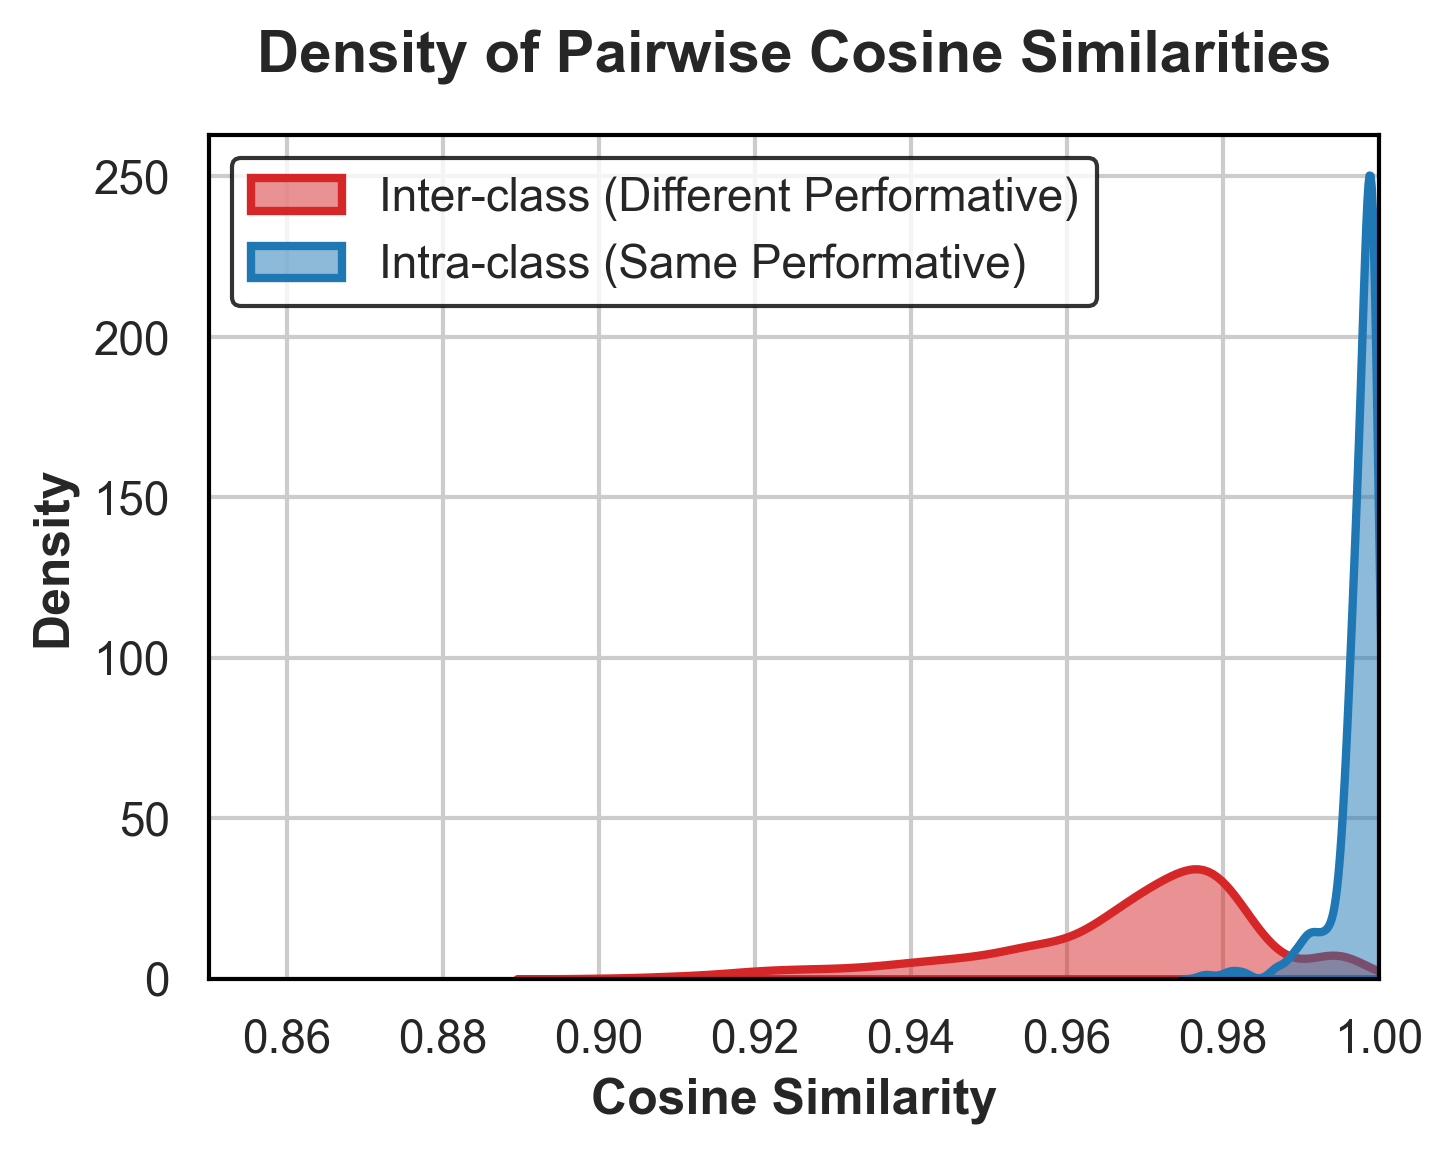
\includegraphics[width=\textwidth]{images/NLP/similarity/kde.png} 
        \caption{Cosine similarity distributions. The high inter-performative similarity (red) indicates severe class overlap, while the narrow intra-performative spread (blue) shows poor target separation.}
    \end{subfigure}
    \hfill
    % Right side: t-SNE Projection
    \begin{subfigure}[b]{0.48\textwidth}
        \centering
        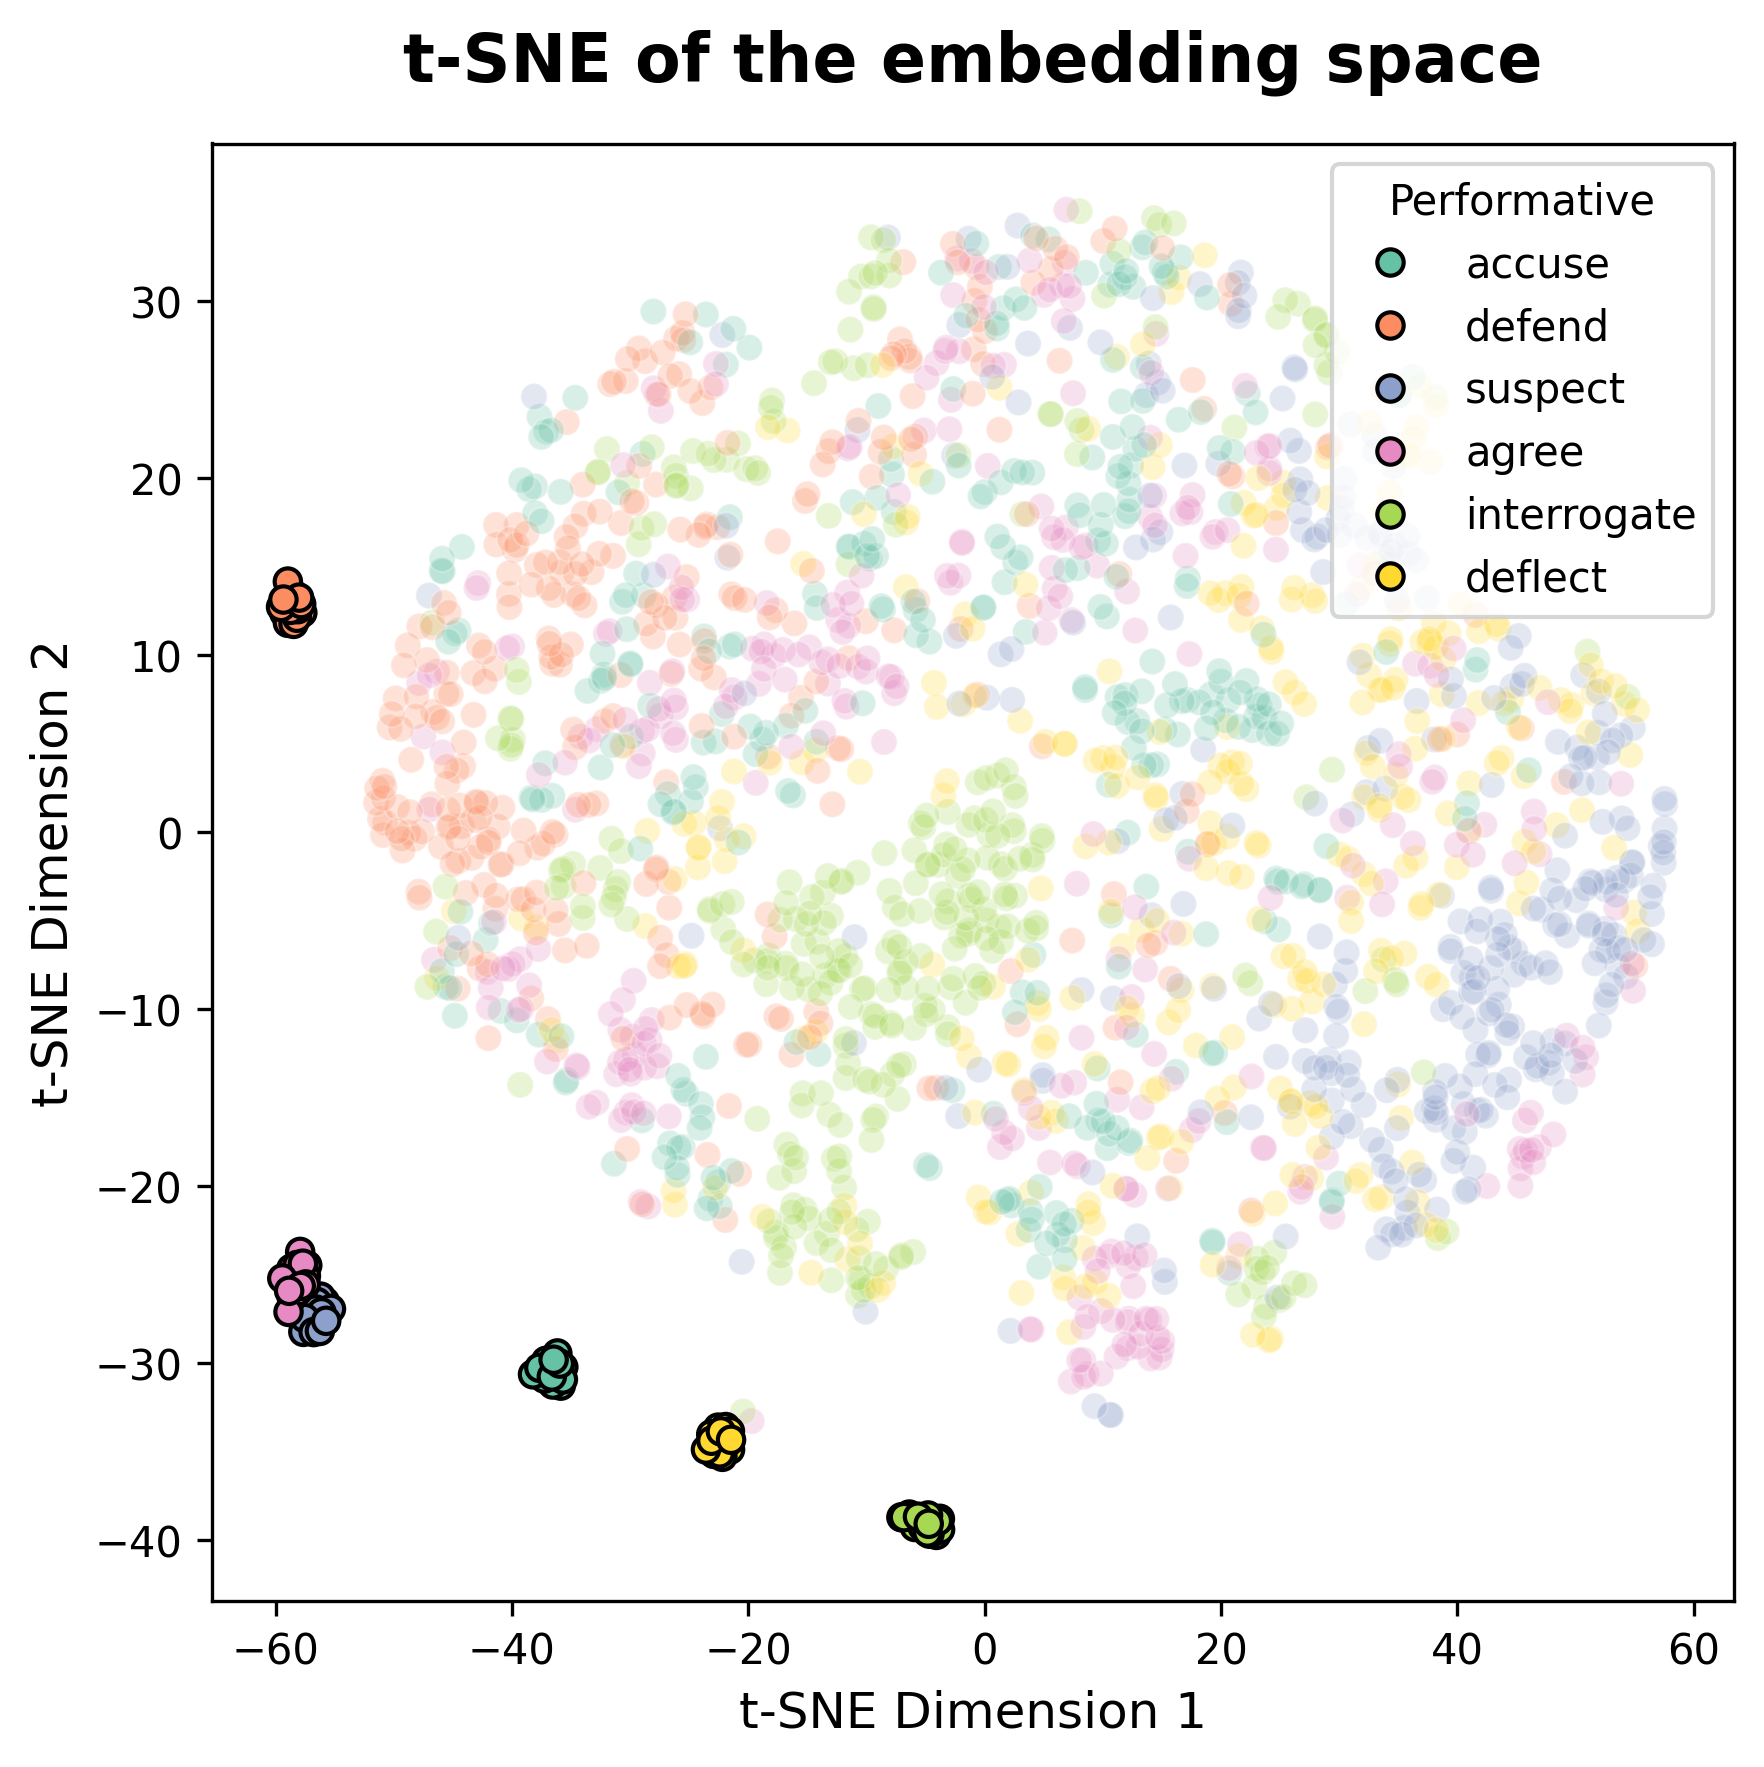
\includegraphics[width=\textwidth]{images/NLP/similarity/tsne_anchor.png} 
        \caption{t-SNE visualization of the embedding space, demonstrating an unstructured manifold with no distinct performative clustering.}
    \end{subfigure}
    \label{fig:tsne_clustering}
    
    \caption{Latent space analysis of raw \texttt{bert-base-uncased} embeddings.}
    \label{fig:clustering_anchors}
\end{figure}

As illustrated in Figure \ref{fig:clustering_anchors}, an analysis of the latent space immediately disproves this hypothesis. The raw \texttt{bert-base-uncased} embeddings fail to naturally cluster pragmatic intent or entity targets. 

Quantitative evaluation on the test dataset confirms this structural failure. By assigning each test message to the label of its nearest anchor, the baseline model achieved an accuracy of only \textbf{22.22\%} for performative prediction and \textbf{8.02\%} for target prediction. This demonstrates that raw BERT representations are insufficiently structured to capture complex speech acts without task-specific fine-tuning.



\subsection{Baseline 2: Non-Linear Classification via Gaussian Kernel}

While the linear similarity baseline failed, the t-SNE projection (Figure \ref{fig:clustering_anchors}) indicated the presence of non-linearly separable structures within the embedding space. To exploit this, we extracted the dense 768-dimensional vectors from the frozen \texttt{bert-base-uncased} model and utilized them directly as the input feature space for a Support Vector Machine (SVM). To capture the complex relations between intents and targets, we applied a Gaussian Radial Basis Function (RBF) kernel; it implicitly maps the features to handle non-linear separations, which significantly improved classification performance over the linear baseline.

\begin{figure}[H]
    \centering
    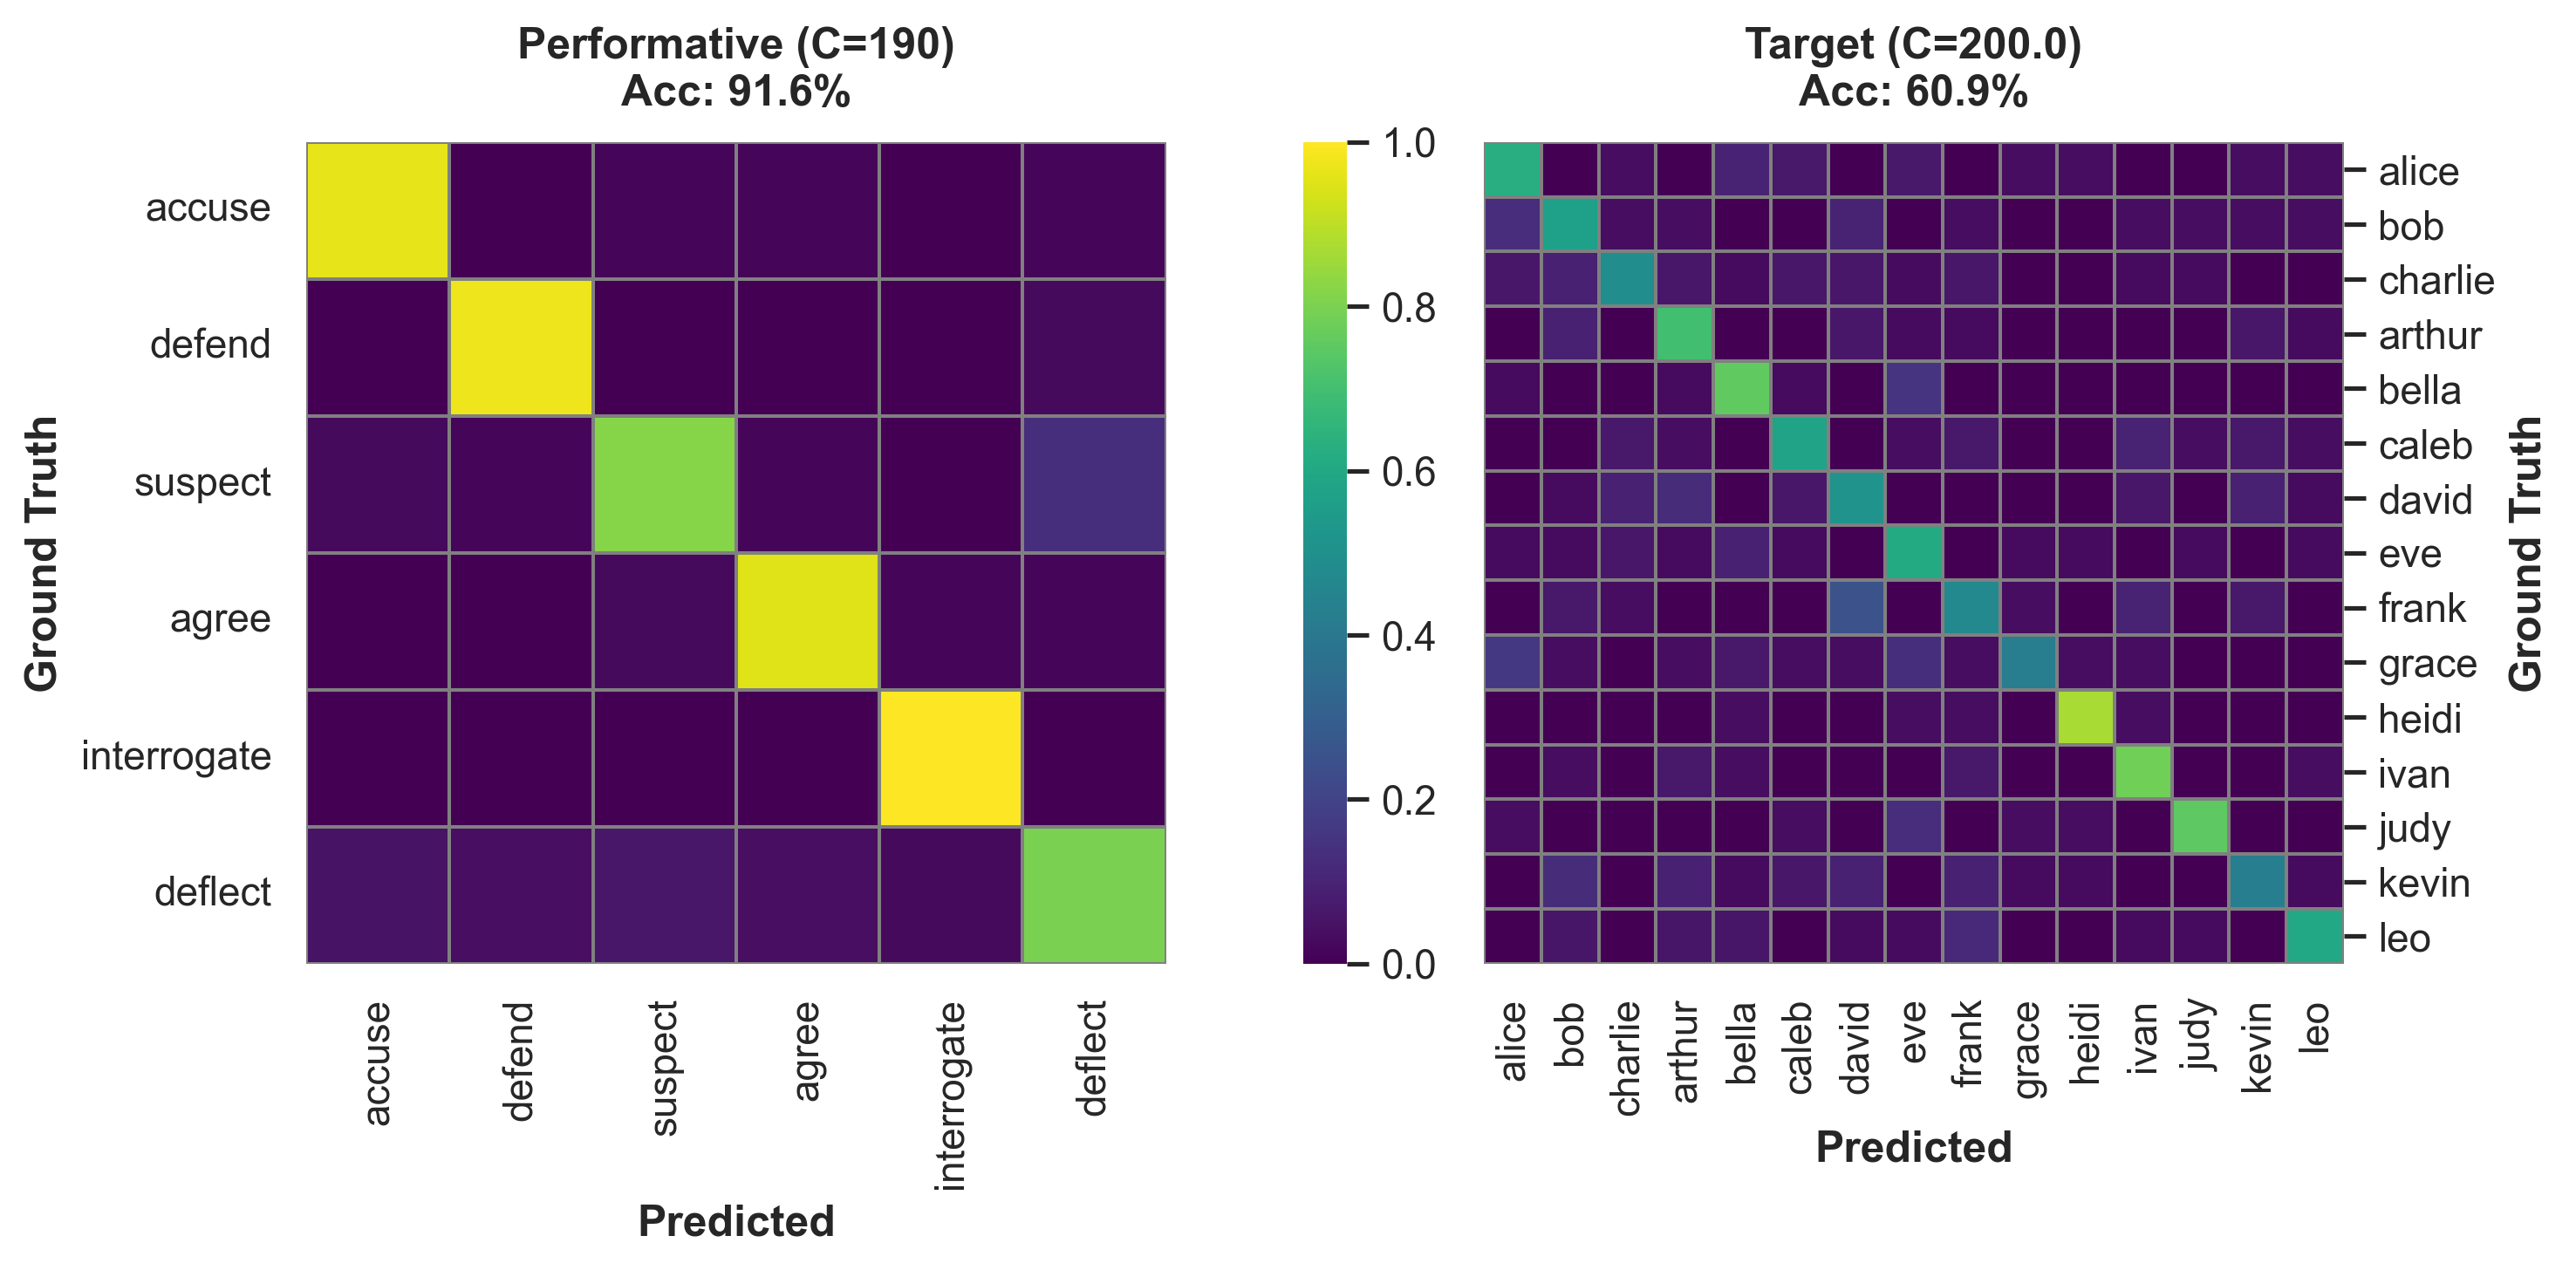
\includegraphics[width=1\textwidth]{images/NLP/kernel/cm_combined.png}
    \caption{Confusion matrices demonstrating improved classification performance for performatives and targets using a Gaussian RBF kernel on frozen BERT embeddings.}
    \label{fig:bert_kernel}
\end{figure}

Despite the improved accuracy, this methodology exhibits severe computational and architectural flaws. First, kernel-based classifiers scale quadratically ($\mathcal{O}(N^2)$), rendering real-time inference too slow and memory-intensive for an active dialogue agent. Second, relying on frozen, generic dense embeddings fails to capture task-specific semantics. Specifically, the low target classification accuracy (60.2\%) proves that a general-purpose BERT model inherently lacks the specialized representation needed to isolate these specific game entities. 

Therefore, to achieve scalable inference and explicitly force the latent space to mathematically disentangle pragmatic intent from target entities, an end-to-end fine-tuned neural architecture is required.


\subsection{Custom Architecture: Joint Fine-Tuning}

To overcome the limitations of frozen representations, we implemented an end-to-end fine-tuned architecture. For comparative consistency, the backbone remains the \texttt{bert-base-uncased} model. The 768-dimensional \texttt{pooler\_output} is routed into two parallel, task-specific classification heads. Each head is structured as a Multi-Layer Perceptron (MLP) consisting of a linear dimensionality reduction (halving the hidden dimension to 384), a ReLU activation, a dropout layer, and a final linear projection to the respective class logits.

The custom model was fine-tuned end-to-end utilizing the Adam optimizer with a learning rate of $\eta = 2 \times 10^{-5}$ and a batch size of 256. To simultaneously optimize for both intent and entity recognition, the network minimized a joint objective function formulated as the unweighted sum of the categorical cross-entropy losses from the performative and target classification heads:
$$ \mathcal{L}_{total} = \mathcal{L}_{perf} + \mathcal{L}_{target} $$
The optimization process was executed for a total of 800 global steps, with validation loss monitored at regular intervals to capture the optimal weights and ensure convergence without overfitting.

\begin{figure}[H]
    \centering
    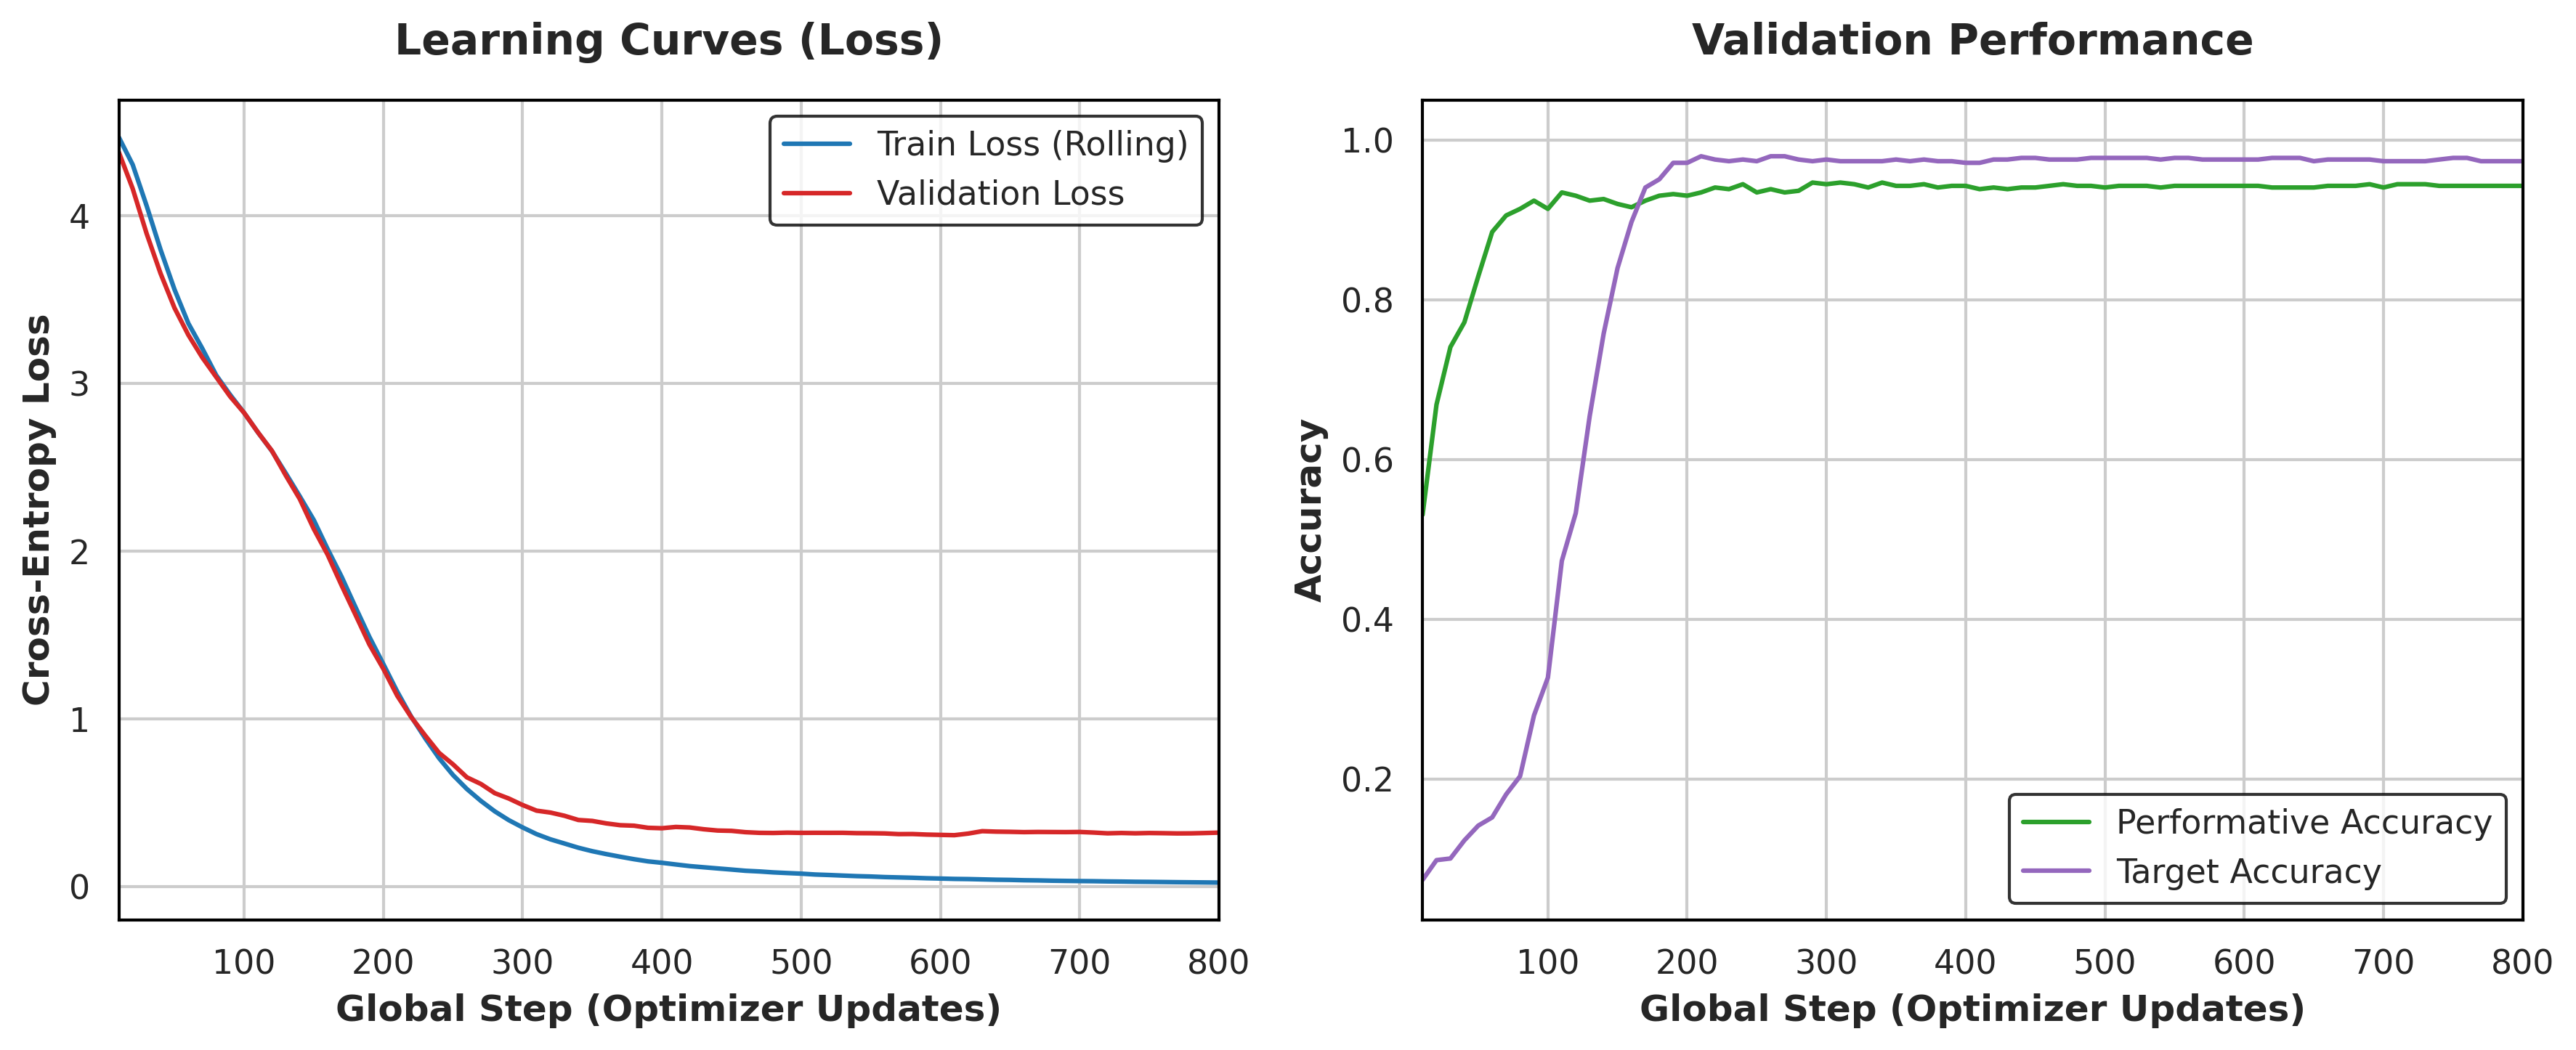
\includegraphics[width=1\textwidth]{images/NLP/finetuning/plot_train.png}
    \caption{Training and validation loss curves. The right panel illustrates the distinct validation losses for the performative and target classification heads.}
    \label{fig:finetuning_loss}
\end{figure}

As illustrated in Figure \ref{fig:finetuning_loss}, the joint optimization achieved near-perfect validation accuracy after ~2 minutes of training on a single NVIDIA RTX 5090. The performative head converged rapidly, consistent with the earlier observation that intent classification relies on broader, easily captured syntactic structures. Conversely, the target head required more updates to converge but ultimately achieved superior final performance. This aligns with our Closed World Assumption: once the network learns to isolate the explicit entity names, target classification reduces to a highly deterministic token lookup.

\begin{figure}[H]
    \centering
    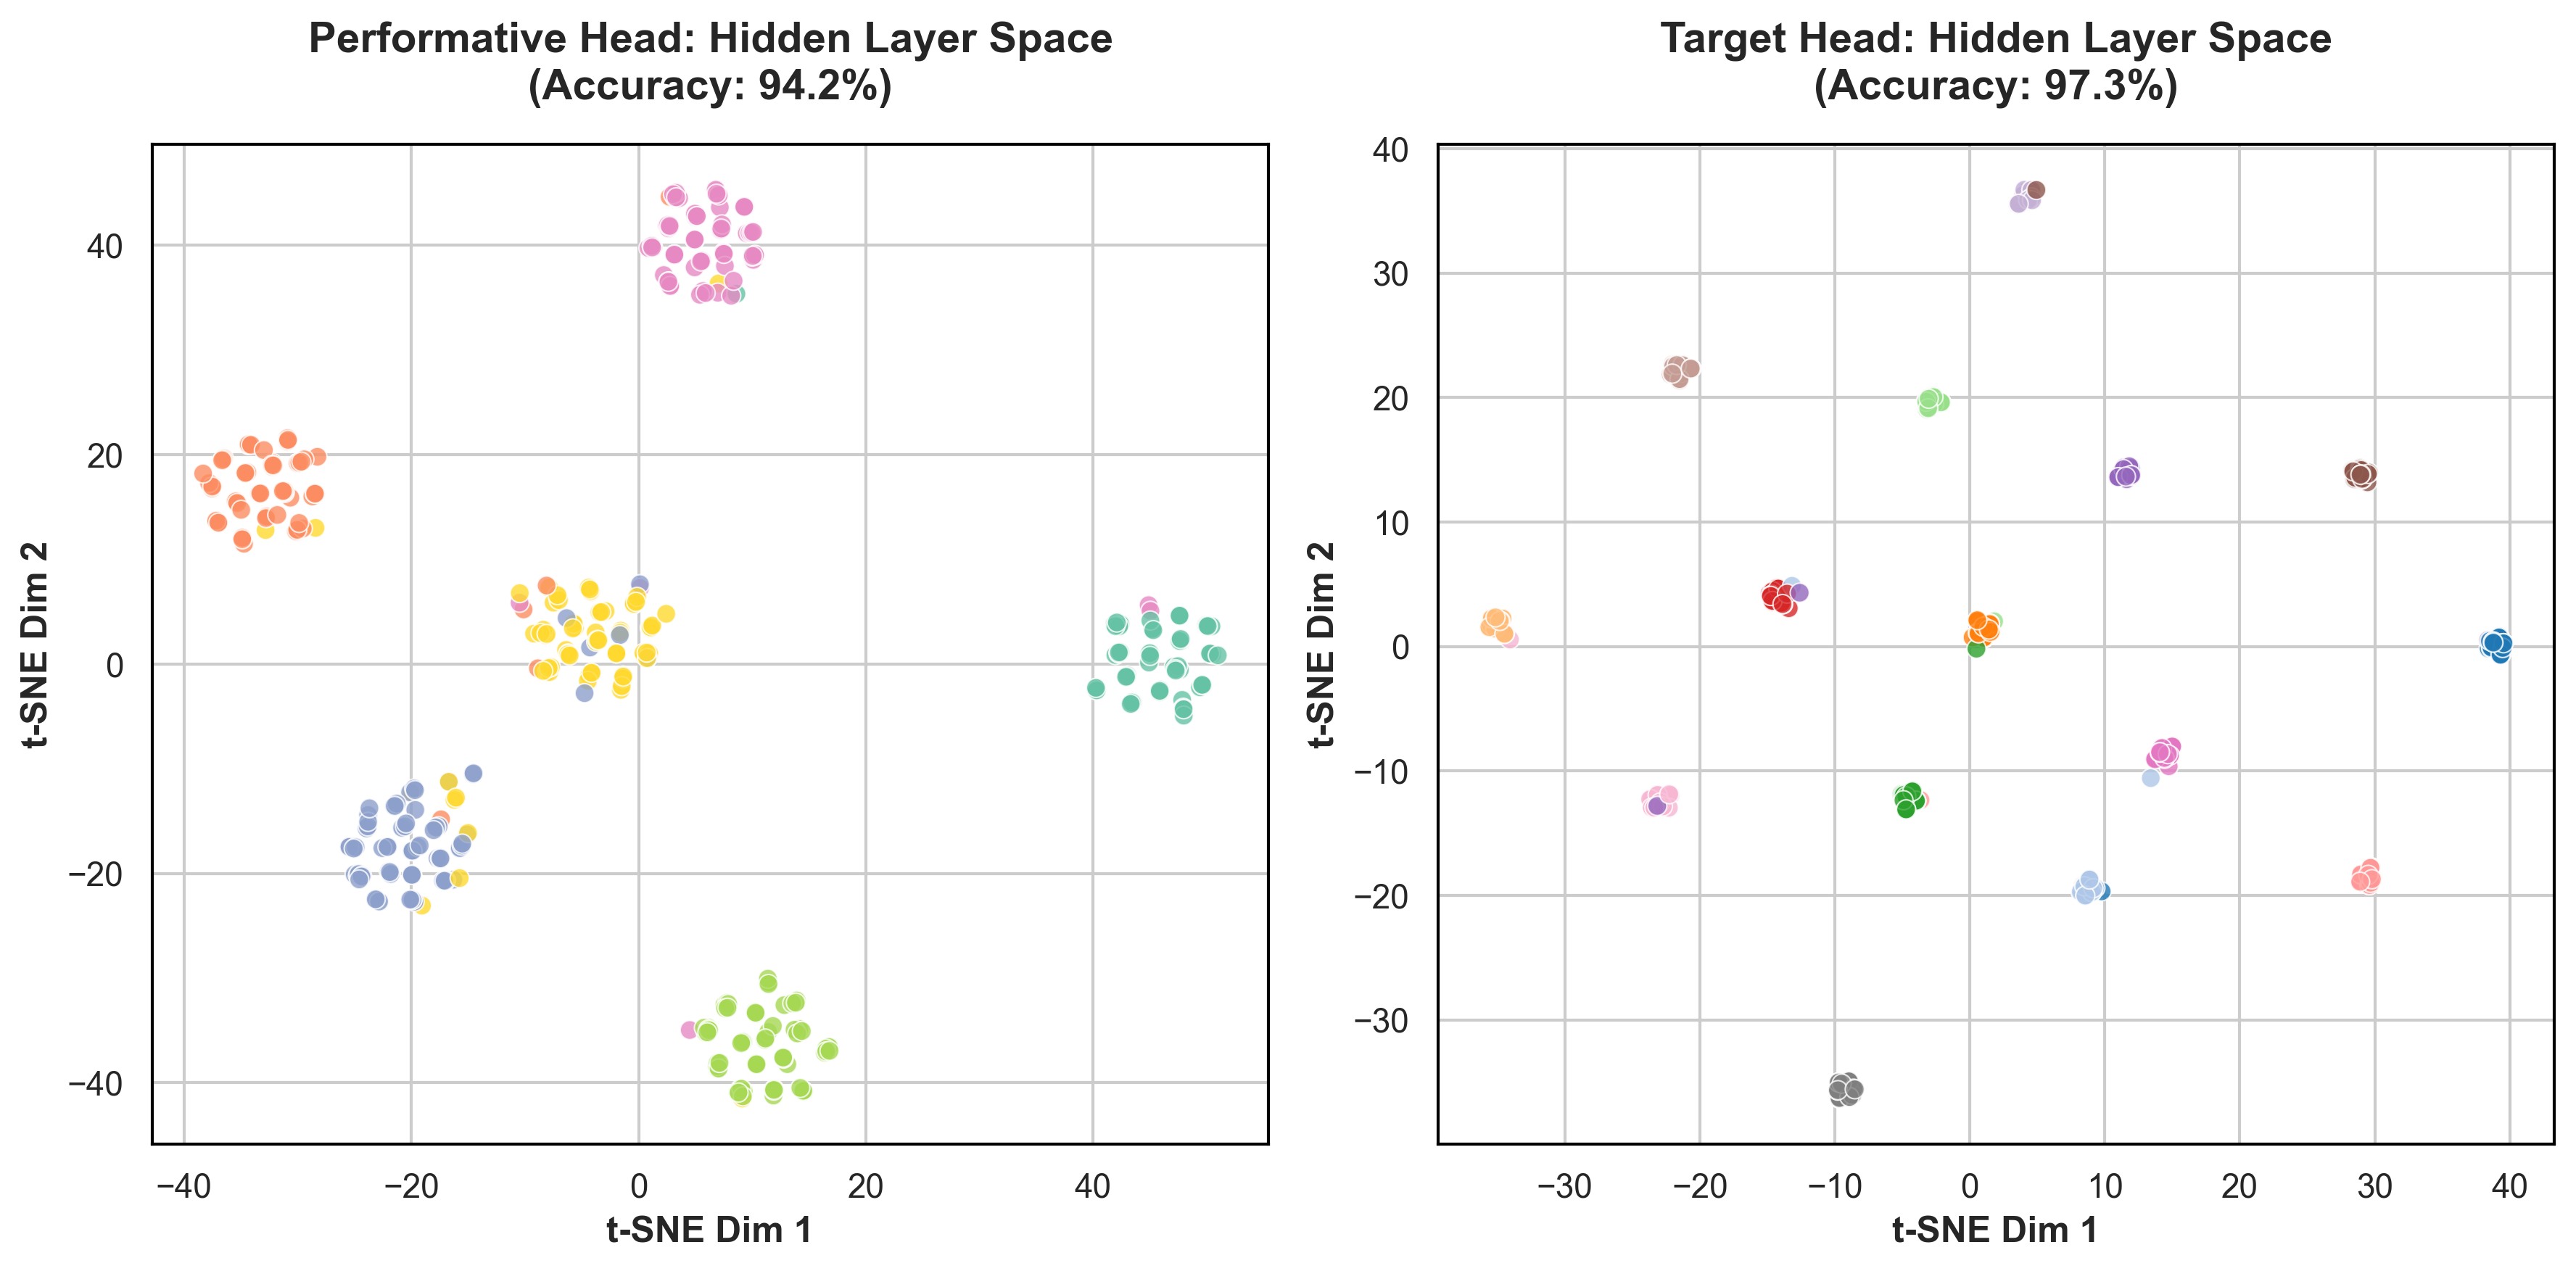
\includegraphics[width=1\textwidth]{images/NLP/finetuning/plot_heads_tsne.png}
    \caption{t-SNE projections of the hidden layers from both classification heads (evaluated on the validation set), demonstrating perfect structural clustering.}
    \label{fig:finetuning_tsne}
\end{figure}

Figure \ref{fig:finetuning_tsne} geometrically confirms this success. By extracting the hidden representations immediately following the ReLU activations of each head, the t-SNE projection proves that the network successfully warps the shared BERT manifold into two distinctly clustered, task-specialized geometric spaces.

To validate the model's real-world robustness, we deployed the fine-tuned architecture on the unbalanced test sets representing actual simulated gameplay, in the test set cited before.

\begin{figure}[H]
    \centering
    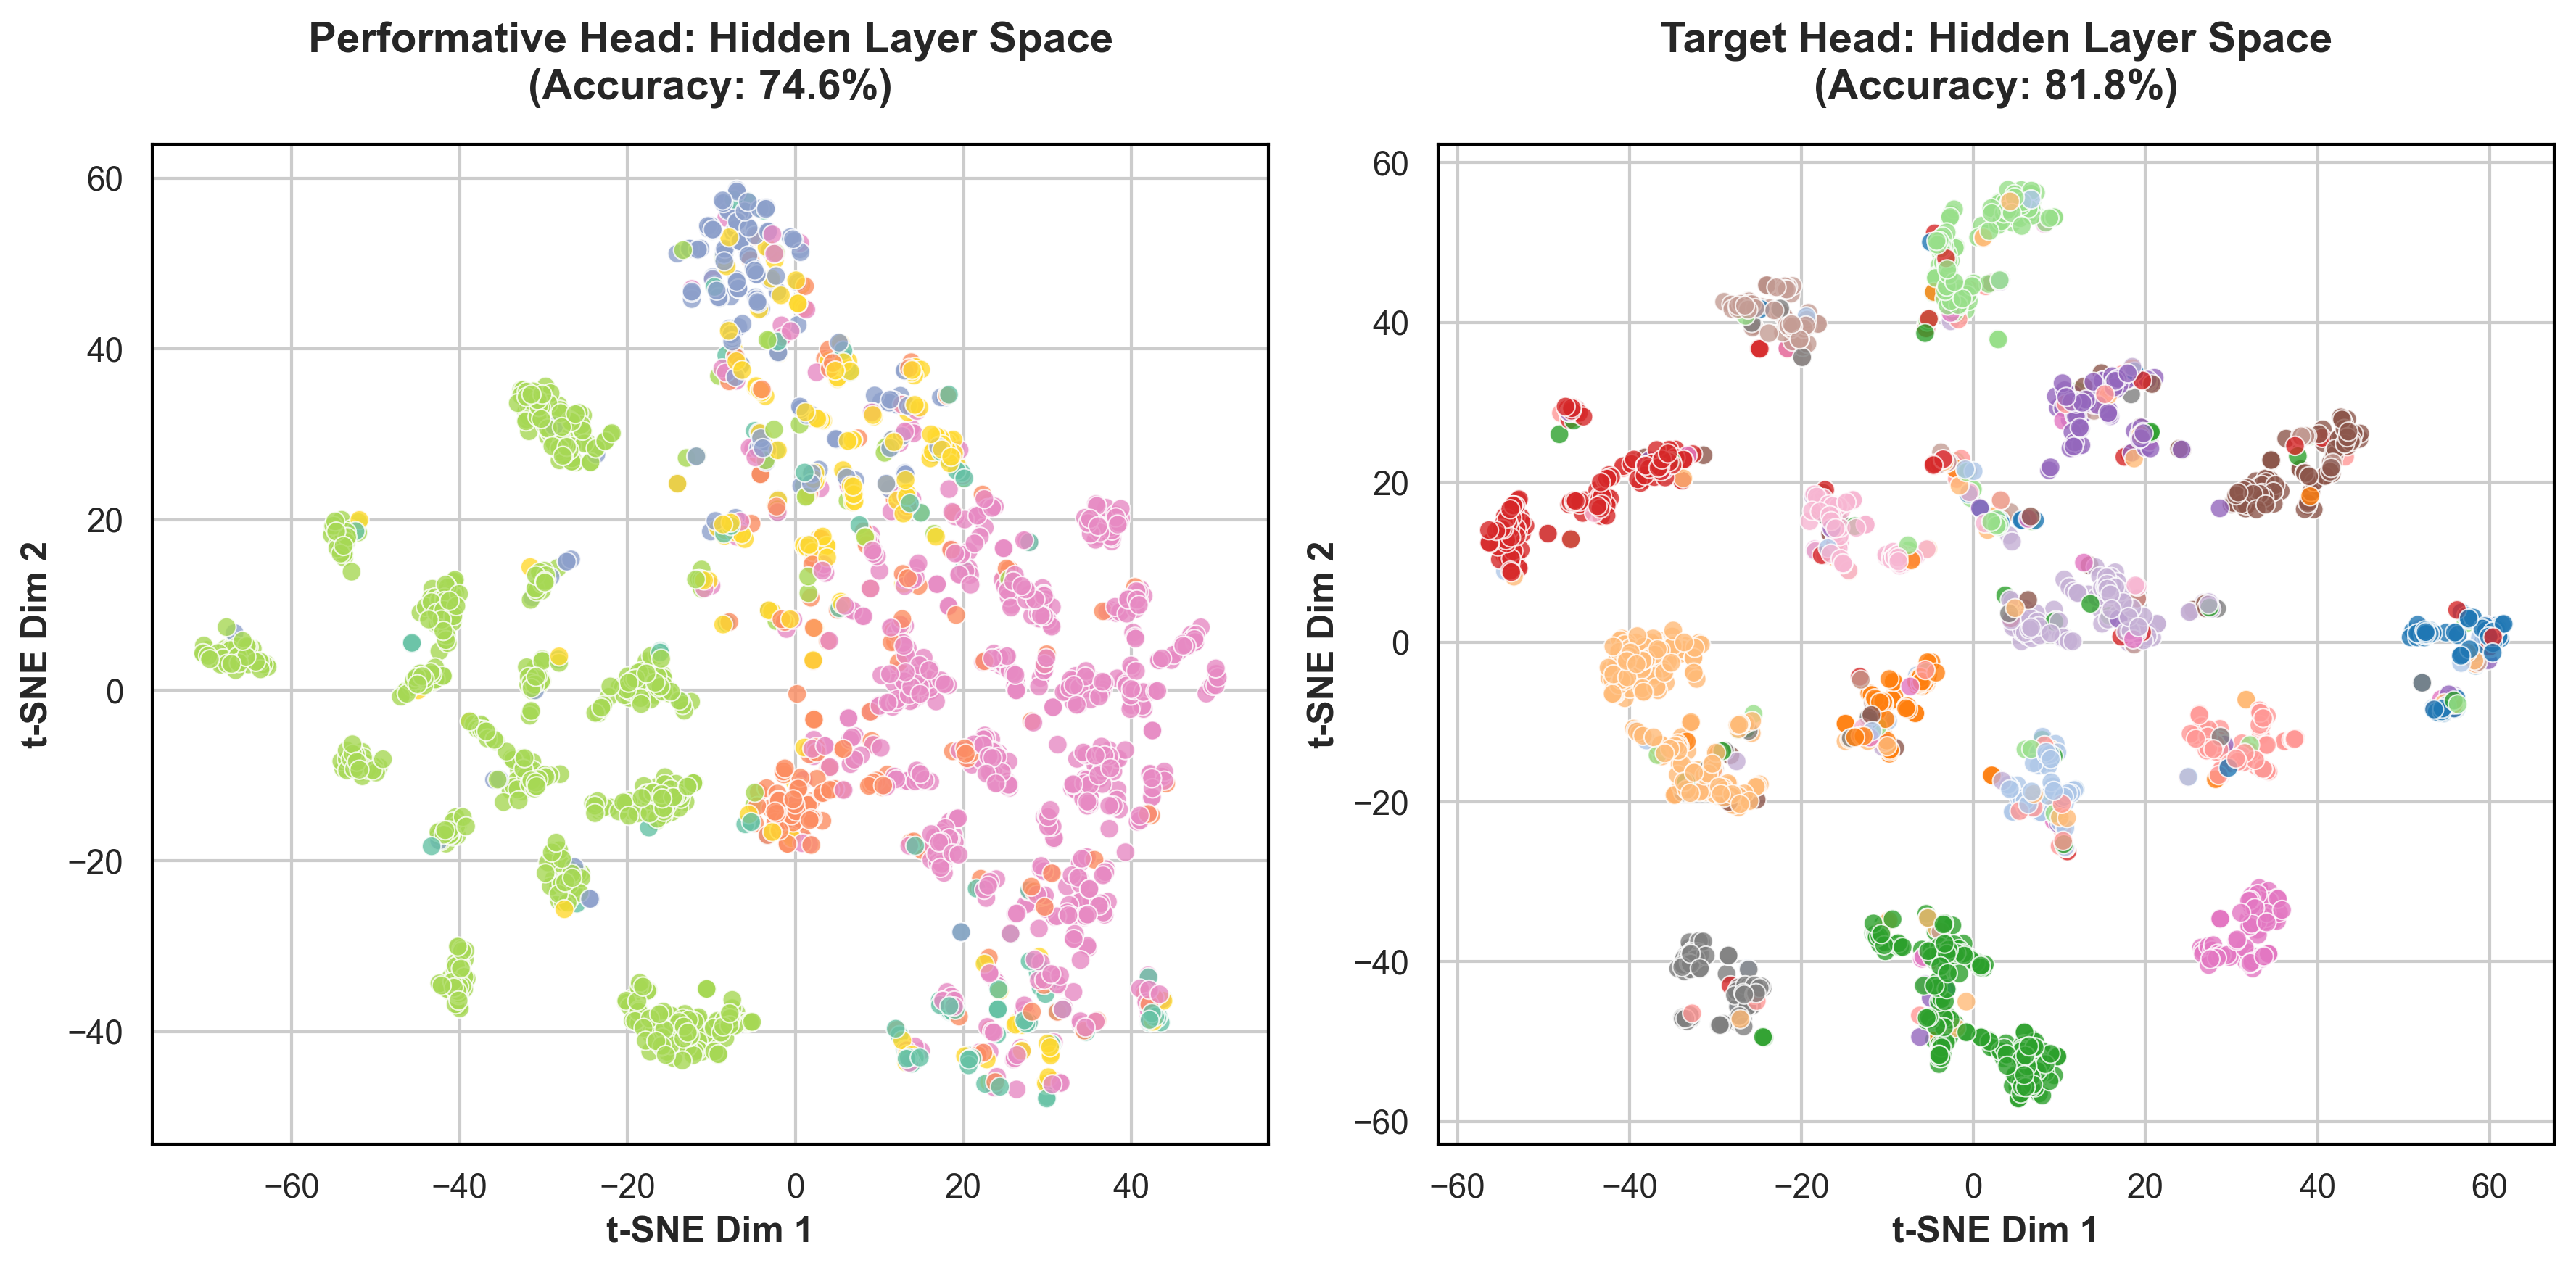
\includegraphics[width=1\textwidth]{images/NLP/finetuning/test_domain_adaptation.png}
    \caption{t-SNE projections of the hidden layers evaluated on the cross-model test set (\texttt{Qwen3.5:35b}). The disintegration of the previously distinct clusters visually explains the degradation in classification performance due to domain shift.}
    \label{fig:finetuning_domain_adaptation_tsne}
\end{figure}

While the model maintained high accuracy on the in-distribution test set, the cross-model evaluation revealed a critical vulnerability to domain shift. Figure \ref{fig:finetuning_domain_adaptation_tsne} illustrates the geometric impact of processing the \texttt{Qwen3.5:35b} dataset. Unlike the perfectly segregated manifold observed during validation (Figure \ref{fig:finetuning_tsne}), the cross-model latent space exhibits severe structural collapse and overlapping decision boundaries. This manifold degradation provides direct geometric proof for the drop in classification performance: the \texttt{SimpleJointBERT} architecture partially overfit the specific lexical and syntactic artifacts of \texttt{Gemma4:31b}, failing to robustly generalize the extraction of pragmatic intent from the phrasing of an unseen generator.


\subsection{Results Summary}

Table \ref{tab:results_summary} provides a comprehensive quantitative comparison of all evaluated methodologies. The progression demonstrates the structural inability of frozen representations to capture pragmatic semantics, contrasted with the high efficacy and deterministic target-lookup capability of the end-to-end fine-tuned custom architecture.

\begin{table}[H]
    \centering
    \resizebox{\textwidth}{!}{
        \begin{tabular}{llcc}
            \hline
            \textbf{Technique} & \textbf{Dataset} & \textbf{Performative Acc. (\%)} & \textbf{Target Acc. (\%)} \\
            \hline
            Naive Baseline & --- & 16.67 & 6.67 \\
            Anchor-Based Classification & Validation & 22.22 & 8.02 \\
            SVM (Gaussian RBF) & Validation & 91.60 & 60.90 \\
            \hline
            \multirow{4}{*}{\texttt{Custom Architecture}} & Training & 100.00 & 100.00 \\
             & Validation & 94.20 & 97.30 \\
             & Test (In-Distribution) & 96.90 & 98.40 \\
             & \textbf{Test (Cross-Model)} & \textbf{74.60} & \textbf{81.80} \\
            \hline
        \end{tabular}
    }
    \caption{Summary of classification accuracies across methodologies and datasets.}
    \label{tab:results_summary}
\end{table}

Lastly, to allows for a run-time use of the model during the games, a python-based microservice (defined in the directory \texttt{BERT\_API}) was implemented, which exposes the fine-tuned model through a REST API. This allows the Jason agents to query the service in real-time during gameplay, providing the raw message text and receiving the predicted performative and target labels for downstream decision-making processes.